\chapter{Material complementario sobre Negatividad}
\label{ap_negatividad}

%CAMBIAR ESTO PARA PERSONALIZARLO A MI GUSTO
\pagestyle{fancy}
\fancyhf{}
\fancyhead[LE]{\nouppercase{\rightmark\hfill}}
\fancyhead[RO]{\nouppercase{\leftmark\hfill}}
\fancyfoot[LE,RO]{\hfill\thepage\hfill}

\begin{figure}
    \centering
    \includegraphics[width=0.8\linewidth]{figuras/ch2/negatividad/3x3 gg2 $N_{01}$ 012 012.png}
    \caption{Negatividad $N_{01}$ para condicion inicial $\ket{gg2}$.}
    \label{fig2:N_01_gg2}
\end{figure}

\begin{figure}
    \centering
    \includegraphics[width=0.8\linewidth]{figuras/ch2/negatividad/3x3 gg2 $N_{02}$ 012 012.png}
    \caption{Negatividad $N_{02}$ para condicion inicial $\ket{gg2}$.}
    \label{fig2:N_02_gg2}
\end{figure}

\begin{figure}
    \centering
    \includegraphics[width=0.8\linewidth]{figuras/ch2/negatividad/3x3 gg2 $N_{12}$ 012 012.png}
    \caption{Negatividad $N_{12}$ para condicion inicial $\ket{gg2}$.}
    \label{fig2:N_12_gg2}
\end{figure}

\begin{figure}
    \centering
    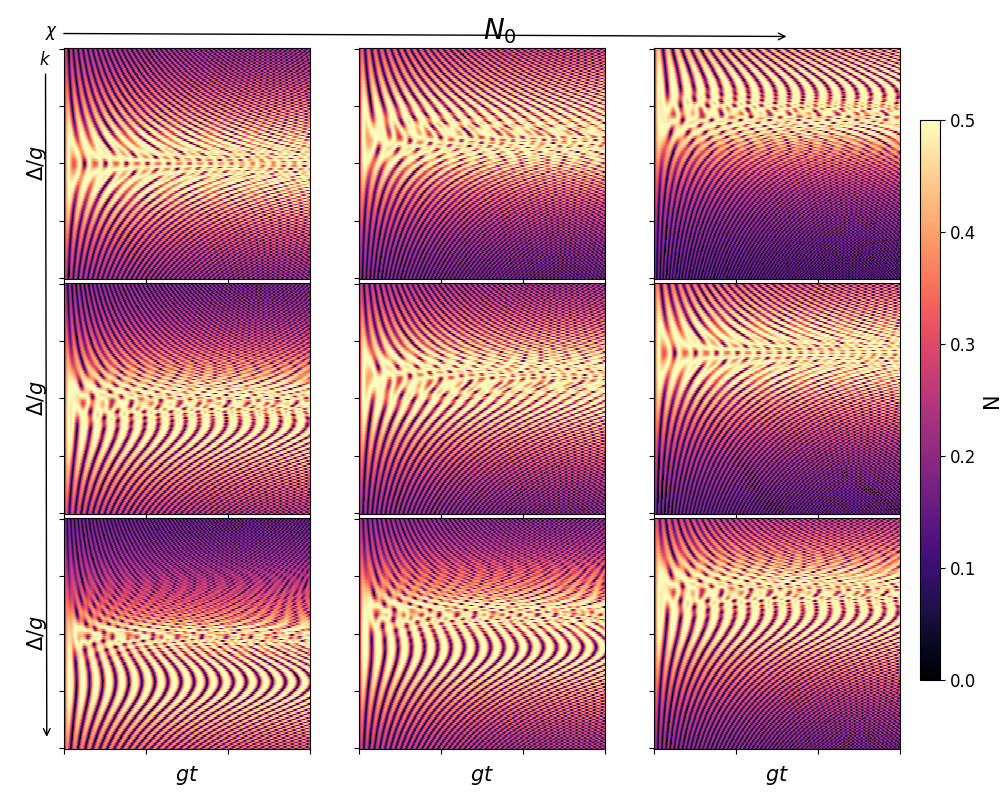
\includegraphics[width=0.8\linewidth]{figuras/ch2/negatividad/3x3 gg2 $N_0$ 012 012.png}
    \caption{Negatividad $N_{0}$ para condicion inicial $\ket{gg2}$.}
    \label{fig2:N_0_gg2}
\end{figure}

\begin{figure}
    \centering
    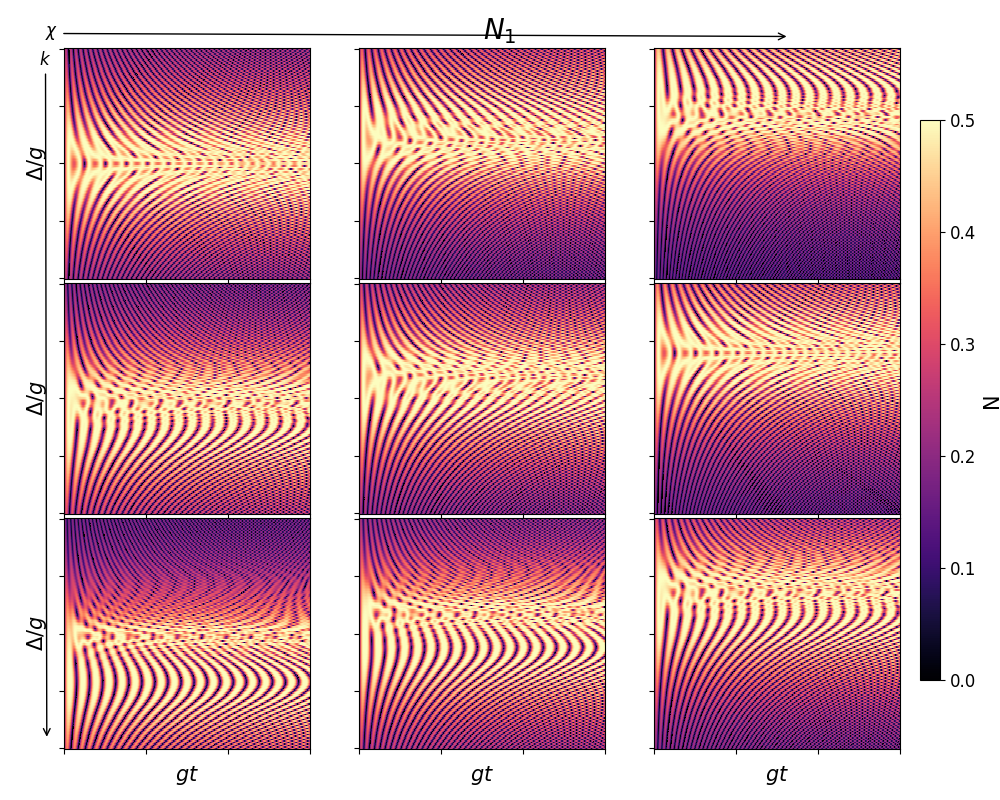
\includegraphics[width=0.8\linewidth]{figuras/ch2/negatividad/3x3 gg2 $N_1$ 012 012.png}
    \caption{Negatividad $N_{1}$ para condicion inicial $\ket{gg2}$.}
    \label{fig2:N_1_gg2}
\end{figure}

\begin{figure}
    \centering
    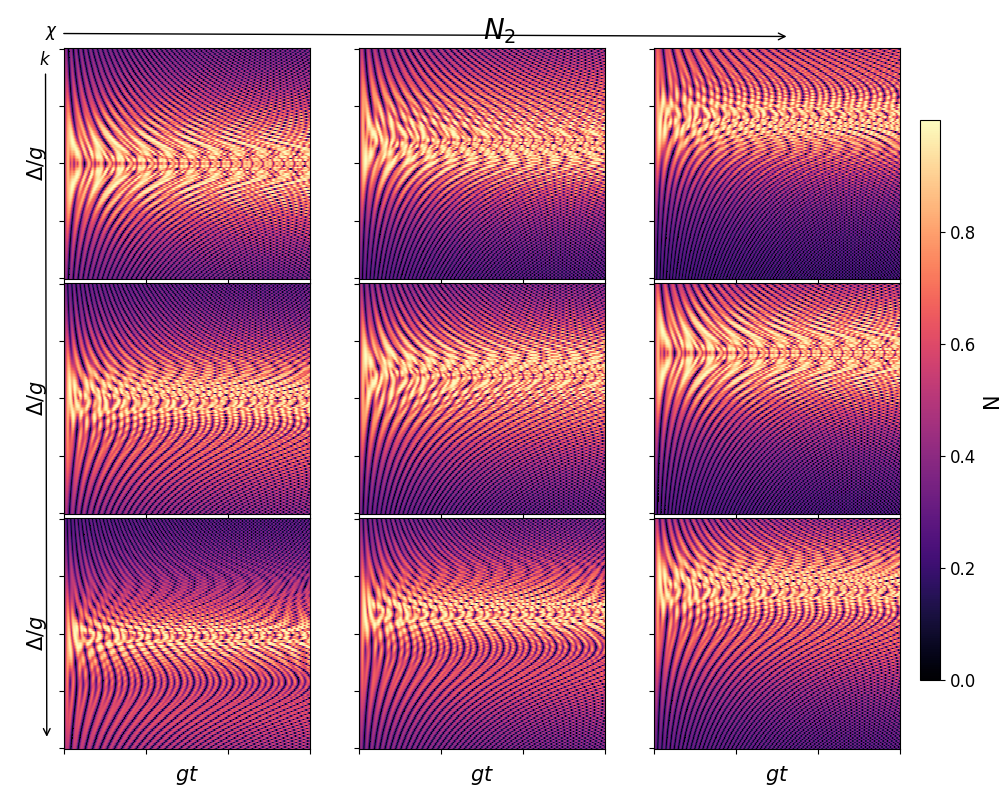
\includegraphics[width=0.8\linewidth]{figuras/ch2/negatividad/3x3 gg2 $N_2$ 012 012.png}
    \caption{Negatividad $N_{2}$ para condicion inicial $\ket{gg2}$.}
    \label{fig2:N_2_gg2}
\end{figure}